 
% Lab 5 for ENGR 1120 030 031 E01 - Tristan Hill - Spring 2016 - Summer 2022
% Introduction to MATLAB 

% Basic Array Operations
% Projectile Motion Example
 
% Document settings
\documentclass[11pt]{article}
\usepackage[margin=1in]{geometry}
\usepackage[pdftex]{graphicx}
\usepackage{multirow}
\usepackage{setspace}
\usepackage{hyperref}
\usepackage{color,soul}
\usepackage{fancyvrb}
\usepackage{framed}
\usepackage{wasysym}
\usepackage{multicol}
\usepackage{gensymb}

\pagestyle{plain}
\setlength\parindent{0pt}
\hypersetup{
    bookmarks=true,         % show bookmarks bar?
    unicode=false,          % non-Latin characters in Acrobat’s bookmarks
    pdftoolbar=true,        % show Acrobat’s toolbar?
    pdfmenubar=true,        % show Acrobat’s menu?
    pdffitwindow=false,     % window fit to page when opened
    pdfstartview={FitH},    % fits the width of the page to the window
    pdftitle={My title},    % title
    pdfauthor={Author},     % author
    pdfsubject={Subject},   % subject of the document
    pdfcreator={Creator},   % creator of the document
    pdfproducer={Producer}, % producer of the document
    pdfkeywords={keyword1} {key2} {key3}, % list of keywords
    pdfnewwindow=true,      % links in new window
    colorlinks=true,        % false: boxed links; true: colored links
    linkcolor=red,          % color of internal links (change box color with linkbordercolor)
    citecolor=green,        % color of links to bibliography
    filecolor=magenta,      % color of file links
    urlcolor=blue           % color of external links
}

% assignment number 

\newcommand{\VSpaceSize}{2mm} 
\newcommand{\HSpaceSize}{2mm} 
\newcommand{\secNum}{GSET: Programming}
\newcommand{\assnType}{Lab}
\newcommand{\assnTitle}{Array Operations - Graphing Math Functions}
\newcommand{\assnNum}{5} 
\newcommand{\currTerm}{Summer 2022}

\definecolor{mygray}{rgb}{.6, .6, .6}

\setulcolor{red} 
\setstcolor{green} 
\sethlcolor{mygray} 

\begin{document}


    \textbf{\LARGE ENGR \hspace{2mm}\secNum \hspace{3mm} \currTerm} \\\\
    \textbf{\LARGE \assnType \hspace{1mm}  \assnNum : \assnTitle}

    \begin{description}
        
        \item [\textbf{Overview}]\textbf{:} \\
        
            You have been working with arrays (1-D) to store groups of numbers. Now we will learn to use the some basic array operations in MATLAB. These are known as the {\it element-wise} operations. Keep in mind, these are very different than the typical mathematical operators that you are familiar with.

	\item [\textbf{Scalar Operations}]\textbf{:} 
	
	All of the math we have done so far has been {\it Scalar Arithmetic}. This means that each operand was a Scalar (1x1) and each numerical expression was evaluated as a Scalar (1x1). \\
	
	 \scalebox{1.5}{{\fontfamily{qcr}\selectfont  x=10*2\hspace{20mm}\color{red}--> 20}} \\\\
	  \scalebox{1.5}{{\fontfamily{qcr}\selectfont  y=x*5\hspace{20mm}\color{red}--> 100}} \\
	  
	  \scalebox{1.5}{{\fontfamily{qcr}\selectfont  A=[10, 15, 12, 13]}} \\\\
	  \scalebox{1.5}{{\fontfamily{qcr}\selectfont  p=A(1)*A(3)\hspace{20mm}\color{red}--> 120}} \\
		
	
	\item [\textbf{Element-Wise Operations}]\textbf{:} \\
	
	It is often useful to operate on an entire array at once. Today we will learn 3 new operations for 1D arrays. These operate on the array operands one element at time and generate a array that is the same size and shape as the array operand.
	\begin{itemize}
		\item Element Wise Multiply \scalebox{1.8}{{\fontfamily{qcr}\selectfont  .*}} \\
		\item Element Wise Divide \scalebox{1.8}{{\fontfamily{qcr}\selectfont  ./}} \\
		\item Element Wise Power \scalebox{1.8}{{\fontfamily{qcr}\selectfont  .\^{}}} \\
		
			\scalebox{1.5}{{\fontfamily{qcr}\selectfont  A=[10, 15, 12, 13]}} \\\\
			\scalebox{1.5}{{\fontfamily{qcr}\selectfont  B=[1, 5, 2, 3]}} \\\\
			\scalebox{1.5}{{\fontfamily{qcr}\selectfont  C=A.*B\hspace{20mm}\color{red}--> 10,    75,    24,    39}} \\\\
			\scalebox{1.5}{{\fontfamily{qcr}\selectfont  C=A./B\hspace{20mm}\color{red}-->10.0,    3.0,    6.0,  4.3}} \\\\
			\scalebox{1.5}{{\fontfamily{qcr}\selectfont  C=A.\^{}B\hspace{20mm}\color{red}--> 10, 759375, 144      , 2197}} \\\\
	\end{itemize}
	
	\item [\textbf{ \Large The Curves}] \textbf{ \Large :}
	 \begin{itemize}
	 	\item First Order Polynomial - \scalebox{1.5}{$y=mx+b$}\\
	 	\item Second Order Polynomial - \scalebox{1.5}{$y=Ax^2+Bx+C$}\\
	 	\item Third Order Polynomial - \scalebox{1.5}{$y=Dx^3+Ex^2+Fx+G$} \\
	 	
	 	\item Exponential - \scalebox{1.5}{$y=H\times e^{Ix}$}\\
	 	\item Logarithmic - \scalebox{1.5}{$y=J\times ln(Kx)$}\\
	  \end{itemize}
       
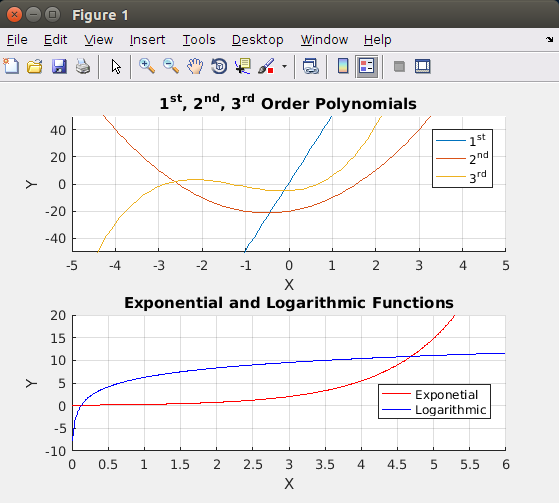
\includegraphics[scale=1]{lab5_fig1.png}\\

	\newpage
	\item [\textbf{ \Large Assignment}] \textbf{ \Large : You are going to write a program to graph the curves shown on the previous page. Your curves do not have to be exactly like mine, but I need to able to identify them. }\\
	\Large
        \begin{enumerate}

	
	
	\item Initialize an array to represent your {\it Independent Variable}. You can see the needed range on the figures shown below. Make sure to use an increment that is small enough to make your curves smooth.\\
		
	\item Compute the dependent values (y -values) for each curve. Make sure  to use the {\it element-wise} operators when you need them and regular operators when you don't.  \\
		
	\item Graph the first, second and, third order polynomials together on figure 1. Each needs it's own line type and color. \\

	\item Graph the exponential and logarithmic curves together on figure 2. Each needs it's own line type color.\\
 
	\item Set the axis of your graphs to ones shown in the example figures.\\
	
 	\item Experiment to find coefficient values that make your figures look similar to mine. They do not have to be perfect.\\
	
	\item Add a title and a legend to both figures.\\
	
	\item Show both figures in a {\it Subplot}.\\
	
	\item Bonus: Show the {\it roots of the polynomials} on figure 1 as visible points with markers.\\
	
        \end{enumerate}
    
    %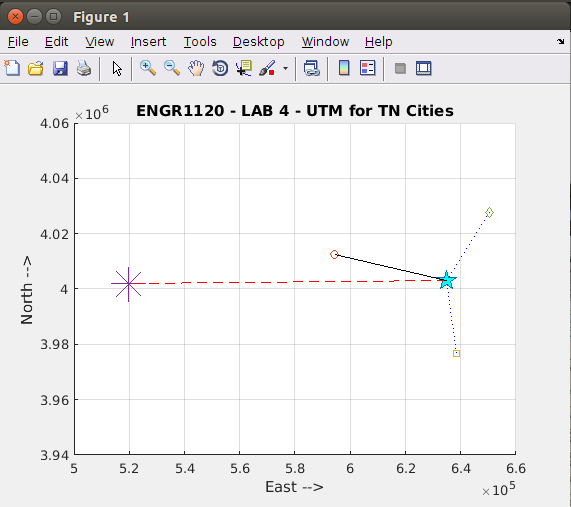
\includegraphics[scale=1]{lab4_fig2.png}

            

        \end{description}
 
\end{document}



